\documentclass[border=12pt]{standalone}
\def\pgfsysdriver{pgfsys-dvisvgm.def}
\usepackage[dvisvgm]{xcolor}
\usepackage{xeCJK}
\setCJKmainfont{HaranoAjiGothic-Regular.otf}[BoldFont=HaranoAjiGothic-Bold.otf]
\setCJKsansfont{HaranoAjiGothic-Regular.otf}[BoldFont=HaranoAjiGothic-Bold.otf]
\usepackage{amsmath,amssymb,tikz,lmodern}
\usetikzlibrary{arrows.meta,positioning,calc,fit,backgrounds}
\renewcommand{\familydefault}{\sfdefault}
\definecolor{ink}{HTML}{25322F}
\definecolor{green}{HTML}{246657}
\definecolor{tint}{HTML}{EEF4F0}
\definecolor{soft}{HTML}{C6D2CC}
\definecolor{muted}{HTML}{52615B}
\newif\ifJapanese
\newcommand{\Tx}[2]{\ifJapanese #1\else #2\fi}
\newcommand{\Eff}{\overline{\operatorname{Eff}}}
\newcommand{\heading}[3]{{\color{green}\bfseries #1\quad\Tx{#2}{#3}}\\[5pt]}
% A white rectangle makes the complete citation label clickable, including spaces.
\newcommand{\refurl}[2]{\special{dvisvgm:raw <a xlink:href="#1" target="_blank" rel="noopener noreferrer">}{\setlength{\fboxsep}{0pt}\colorbox{white}{\color{green}\underline{\strut #2}}}\special{dvisvgm:raw </a>}}
\newcommand{\refedge}[3]{\refurl{\csname source#1\endcsname\string##page=#2}{#3}}
\newcommand{\SF}[2]{\refedge{sf}{#1}{#2}}
% GitHub's file preview does not support PDF page fragments.
\newcommand{\LA}[2]{\refurl{\sourcela}{#2}}
\newcommand{\Sch}[2]{\refedge{sch}{#1}{#2}}
\newcommand{\PS}[2]{\refedge{ps}{#1}{#2}}
\tikzset{
 card/.style={draw=soft,fill=white,rounded corners=2pt,align=left,text=ink,font=\fontsize{10.5}{14}\selectfont,inner xsep=12pt,inner ysep=10pt,text width=14.4cm},
 half/.style={card,text width=6.45cm,minimum height=2.05cm},
 result/.style={card,draw=green,fill=tint,line width=.9pt},
 reason/.style={align=left,text=muted,font=\fontsize{9}{12}\selectfont,inner sep=0pt,text width=12.7cm},
 branchreason/.style={reason,text width=5.95cm},
 edge/.style={-{Stealth[length=2.4mm]},draw=green,line width=1pt},
 wire/.style={draw=green,line width=1pt},
}
% Keep the arrow in a dedicated left gutter; explanations never cover it.
\newcommand{\flow}[3]{
 \coordinate (#2-from) at ($(#1.south)+(-6.9,0)$);
 \coordinate (#2-to) at ($(#2.north)+(-6.9,0)$);
 \draw[edge] (#2-from)--(#2-to);
 \node[reason,anchor=west] (#2-reason) at ($(#2-from)!.5!(#2-to)+(.55,0)$) {#3};
}


\newcommand{\CiteSource}[2]{\refurl{\csname source#1\endcsname}{#2}}

\expandafter\def\csname sourceK4N\endcsname{https://github.com/openai/math/blob/adc7f1241b42e322a6451854ab7e4b4c146bf78a/preprints/Abundance-after-nonvanishing-for-compact-Kahler-fourfolds-September-27-2026/paper.pdf}
\expandafter\def\csname sourceHLL\endcsname{https://arxiv.org/pdf/2508.14634v2}
\expandafter\def\csname sourceDO\endcsname{https://arxiv.org/pdf/2306.00671v4}
\expandafter\def\csname sourceDHP\endcsname{https://arxiv.org/pdf/2205.12205v3}
\expandafter\def\csname sourceFT\endcsname{https://arxiv.org/pdf/2205.14801v7}
\expandafter\def\csname sourceSai\endcsname{https://arxiv.org/pdf/2204.09026v5}
\expandafter\def\csname sourceSS\endcsname{https://perso.pages.math.cnrs.fr/users/claude.sabbah/MHMProject/mhm_chap16.pdf}
\expandafter\def\csname sourceFG\endcsname{https://www.math.kyoto-u.ac.jp/~fujino/fg-comp-final.pdf}
\expandafter\def\csname sourceSL\endcsname{https://github.com/openai/math/blob/adc7f1241b42e322a6451854ab7e4b4c146bf78a/preprints/Lifting-sections-from-the-reduced-support-of-an-adjoint-September-27-2026/paper.pdf}
\expandafter\def\csname sourceLA\endcsname{https://github.com/openai/math/blob/adc7f1241b42e322a6451854ab7e4b4c146bf78a/preprints/Log-abundance-in-characteristic-zero-September-24-2026/paper.pdf}

\Japanesetrue
\begin{document}
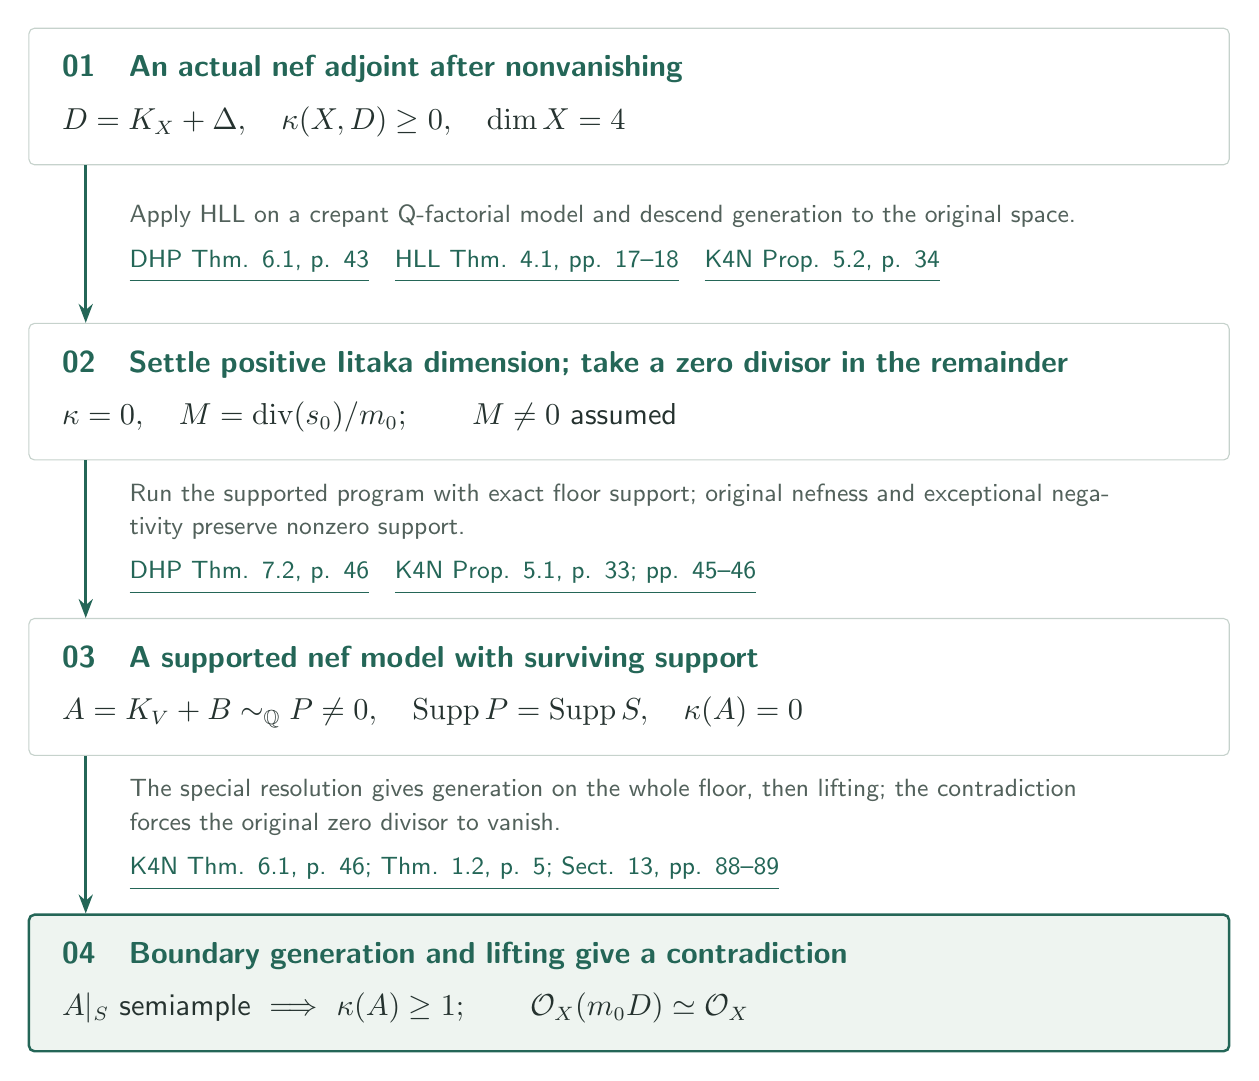
\begin{tikzpicture}
\node[card] (n0) {\heading{01}{非消滅後のnefな実際のadjoint}{An actual nef adjoint after nonvanishing}$D=K_X+\Delta,\quad\kappa(X,D)\geq0,\quad\dim X=4$};
\node[card,below=2.0cm of n0] (n1) {\heading{02}{正の飯高次元を処理し、残りで零因子を取る}{Settle positive Iitaka dimension; take a zero divisor in the remainder}$\kappa=0,\quad M=\operatorname{div}(s_0)/m_0;\qquad M\ne0\ \text{assumed}$};
\flow{n0}{n1}{\Tx{crepantなQ-factorialモデルでHLLを適用し、生成を元の空間へ降ろす。}{Apply HLL on a crepant Q-factorial model and descend generation to the original space.}\\[4pt]\CiteSource{DHP}{DHP Thm. 6.1, p. 43}\quad \CiteSource{HLL}{HLL Thm. 4.1, pp. 17--18}\quad \CiteSource{K4N}{K4N Prop. 5.2, p. 34}}
\node[card,below=2.0cm of n1] (n2) {\heading{03}{台が消えないsupported nefモデル}{A supported nef model with surviving support}$A=K_V+B\sim_{\mathbb Q}P\ne0,\quad\operatorname{Supp}P=\operatorname{Supp}S,\quad\kappa(A)=0$};
\flow{n1}{n2}{\Tx{floorに台を合わせるsupported program。元のnefnessと例外negativityで非零台を保つ。}{Run the supported program with exact floor support; original nefness and exceptional negativity preserve nonzero support.}\\[4pt]\CiteSource{DHP}{DHP Thm. 7.2, p. 46}\quad \CiteSource{K4N}{K4N Prop. 5.1, p. 33; pp. 45--46}}
\node[result,below=2.0cm of n2] (n3) {\heading{04}{境界生成と持ち上げの矛盾}{Boundary generation and lifting give a contradiction}$A|_S\ \text{semiample}\ \Longrightarrow\ \kappa(A)\geq1;\qquad\mathcal O_X(m_0D)\simeq\mathcal O_X$};
\flow{n2}{n3}{\Tx{特別な解消で全floorを生成し、次に持ち上げる。矛盾から元の零因子はゼロ。}{The special resolution gives generation on the whole floor, then lifting; the contradiction forces the original zero divisor to vanish.}\\[4pt]\CiteSource{K4N}{K4N Thm. 6.1, p. 46; Thm. 1.2, p. 5; Sect. 13, pp. 88--89}}
\end{tikzpicture}
\end{document}
